\documentclass[margin=0.1cm]{standalone}
\usepackage{ tikz }
\usepackage{ xparse }
\usepackage{../../../macros}

\begin{document}
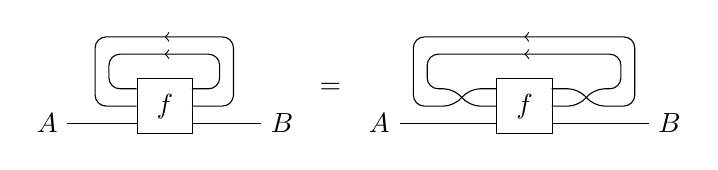
\begin{tikzpicture}[yscale=-1,x=1em,y=1.25em]

    \node at (5,-0.5) {$\null$};

    \node [anchor=east] at (1.5,2) {$A$};
    \node [anchor=west] at (8.5,2) {$B$};

    \draw (1.5,2) -- (4,2);
    \node[draw, minimum height = 2em, minimum width = 2em, anchor = west, fill=white] at (4,1.5){$f$};
    \draw [->, rounded corners] (6,1) -- (7,1) -- (7,0) -- (5,0);
    \draw [rounded corners] (5,0) -- (3,0) -- (3,1) -- (4,1);
    \draw [->, rounded corners] (6,1.5) -- (7.5,1.5) -- (7.5,-0.5) -- (5,-0.5);
    \draw [rounded corners] (5,-0.5) -- (2.5,-0.5) -- (2.5,1.5) -- (4,1.5);
    \draw (6,2) -- (8.5,2);

    \node at (11,1) {$=$};

    \node [anchor=east] at (13.5,2) {$A$};
    \node [anchor=west] at (22.5,2) {$B$};
    
    \draw (13.5,2) -- (17,2);
    \node[draw, minimum height = 2em, minimum width = 2em, anchor = west, fill=white] at (17,1.5){$f$};
    \draw [rounded corners, ->] (19,1) -- (20,1) -- (20.5,1.5) -- (22,1.5) -- (22,-0.5) -- (18,-0.5);
    \draw [rounded corners, ->] (19,1.5) -- (20,1.5) -- (20.5,1) -- (21.5,1) -- (21.5,0) -- (18,0);
    \draw [rounded corners] (18,-0.5) -- (14, -0.5) -- (14, 1.5) -- (15.5, 1.5) -- (16,1) -- (17,1);
    \draw [rounded corners] (18,0) -- (14.5,0) -- (14.5,1) -- (15.5,1) -- (16,1.5) -- (17,1.5);
    \draw (19,2) -- (22.5,2);

\end{tikzpicture}
\end{document}